\documentclass{theme/uniprthesis}

%%%%%%%%%%%Some Extra Packages%%%%%%%%%%%
\usepackage[italian]{babel}		% To have Italina names in Sections, Figures, Chapters etc.
\usepackage{todonotes}			% To ease the revision
\usepackage{blindtext} 			
\usepackage{ifdraft}
\usepackage{afterpage}
\usepackage{amsmath}
\usepackage{amssymb}
\usepackage{amsfonts}
\usepackage{bbold}
\usepackage{lipsum} 
\usepackage{footmisc}
\usepackage{xcolor}
\usepackage{siunitx}
\usepackage{listings}
\usepackage{xcolor}
\usepackage[autostyle=false, style=english]{csquotes}
\MakeOuterQuote{"}
\MakeInnerQuote{ç}


% Stile Python
\lstdefinestyle{mypython}{
  language=Python,
  basicstyle=\ttfamily\small,
  keywordstyle=\color{blue},
  commentstyle=\itshape\color{gray},
  stringstyle=\color{teal},
  showstringspaces=false,
  numbers=left,
  numberstyle=\tiny\color{gray},
  stepnumber=1,
  breaklines=true,
  frame=single,
  tabsize=4
}

%%%%% THESIS / TITLE PAGE INFORMATION
% Everybody needs to complete the following:
\title{Una metodologia computazionale per il riconoscimento di clustering alternativi nella trascrittomica spaziale}
\author{Matteo Cerinelli}
\advisor{Prof. Vincenzo Bonnici}
\college{Dipartimento di Scienze Matematiche, Fisiche e Informatiche}
\degree{Corso di Laurea Triennale in Informatica}
\degreeyears{2024--2025}
\serialNumber{294907}

% Not mandatory fields
\newcommand{\subTitle}{A computational methodology for the recognition of alternative clustering in spatial transcriptomics} %Subtitle, usually the english version of the title

%\newcommand{\advisorSecond}{Prof. Nome2 Cognome2} % For multiple (up to 4) advisors -- if this is not present then also the remaining ones are automatically omitted
%\newcommand{\advisorThird}{Dott. Nome3 Cognome3} % For multiple (up to 4) advisors -- if this is not present then also the remaining ones are automatically omitted
%\newcommand{\advisorFourth}{Dott. Nome4 Cognome4} % For multiple (up to 4) advisors

\newcommand{\coadvisor}{} %For multiple (up to 4) coadvisors -- if this is not present then also the remaining ones are automatically omitted
%\newcommand{\coadvisorSecond}{Prof. co-Nome2 co-Cognome2} % For multiple (up to 4) coadvisors -- if this is not present then also the remaining ones are automatically omitted
%\newcommand{\coadvisorThird}{Dott. co-Nome3 co-Cognome3} % For multiple (up to 4) coadvisors -- if this is not present then also the remaining ones are automatically omitted
%\newcommand{\coadvisorFourth}{Dott. co-Nome4 co-Cognome4} % For multiple (up to 4) coadvisors


\newcommand\blankpage{
    \null
    \thispagestyle{empty}
    \addtocounter{page}{-1}
    \newpage
}

%%%%%%%%%%%%%%%%%%%%%%%%%%%%%%%%%%%%%%%%%%%%%%%%%%%%%%%%%%%%%%%%%%%%%%%%%%%%%%%%%%%%%%%%

\begin{document}

\maketitle
\blankpage % Pagina vuota

%%%%%%%%%%%%%%%%%%%%%%%%%%%%%%%% Citazione
%%%% Commentare questo blocco se non la si vuole mettere
% \newpage
% \thispagestyle{empty}
% \null\vspace{\stretch{1}}
% \begin{flushright}
% 	\textit{Citazione}
% \end{flushright}
% \vspace{\stretch{3}}\null
% \newpage
% \blankpage
%%%%%%%%%%%%%%%%%%%%%%%%%%%%%%%% Fine Citazione

%%%%%%%%%%%%%%%%%%%%%%%%%%%%%%%% Dedica
%%%% Commentare questo blocco se non la si vuole mettere
% \newpage
% \thispagestyle{empty}
% \null\vspace{\stretch{1}}
% \begin{flushright}
% 	\textit{Dedica}
% \end{flushright}
% \vspace{\stretch{3}}\null
% \newpage
% \blankpage
%%%%%%%%%%%%%%%%%%%%%%%%%%%%%%%% Fine Dedica

%%%%%%%%%%%%%%%%%%%%%%%%%%%%%%%% Indici
\pagestyle{plain}
\pagenumbering{arabic}
\tableofcontents

 \listoffigures    % Commentare se non vi sono immagini
 %\listofalgorithms % Commentare se non vi sono algoritmi
 \lstlistoflistings
 \listoftables     % Commentare se non vi sono tabelle

%%%%%%%%%%%%%%%%%%%%%%%%%%%%%%%% Prefazione
%\pagenumbering{arabic}
\chapter{Introduzione}\label{chapter:introduzione} 
Negli ultimi anni la \textit{trascrittomica spaziale} (TS) ha rappresentato una delle innovazioni
più significative nel campo della biologia molecolare e della bioinformatica.  
A differenza delle tecniche di trascrittomica tradizionali, che misurano i livelli di espressione genica senza
informazioni di posizione, in quanto le cellule devono essere estratte dal tessuto, la trascrittomica spaziale consente di mappare l'attività dei geni direttamente nel contesto
del tessuto senza bisogno alcuno di doverle rimuovere.  
Questo approccio fornisce una visione bidimensionale dell'espressione genica, permettendo di studiare
non solo quali geni sono attivi, ma anche la loro posizione spaziale.

La possibilità di associare informazione spaziale all'espressione ha aperto nuove prospettive nello studio dei processi
biologici complessi, come lo sviluppo embrionale, l'organizzazione dei tessuti e la progressione di patologie come i
tumori. Tuttavia, l'analisi di questo tipo di dati presenta notevoli sfide computazionali: la quantità di dati da analizzare
è elevata e le relazioni spaziali tra geni sono intricate, e l'analisi dei cluster spaziali non sempre scova tutti i possibili pattern, spesso scambiando rumore per dati utili o viceversa.  
Da qui nasce la necessità di sviluppare strumenti e algoritmi in grado di integrare informazione geometrica, topologica di espressione al fine di trovare cluster alternativi.

\medskip
Date queste premesse si sviluppa il lavoro presentato in questa tesi, il cui obiettivo principale è stato quello di
progettare e realizzare una pipeline computazionale per l'identificazione e la classificazione delle relazioni spaziali
tra geni in un dataset 10x Visium al fine di trovare cluster spaziali alternativi.  
Partendo dai dati di espressione e dalle coordinate spaziali degli \textit{spot}, è stata costruita una lista degli spot vicini
tramite l'algoritmo dei \textit{Nearest Neighbors} (k-NN), in modo da avere le connessioni spaziali tra i vari spot del tessuto.  
Successivamente, ogni gene è stato suddiviso in \textit{sottogeni}, regioni locali di espressione contigua, mediante
l'individuazione delle \textit{componenti connesse} partendo dalle maschere binarie di espressione genica.  
Questo passaggio ha consentito di confrontare i sottogeni tra loro
e valutare diverse tipologie di rapporto spaziale: sovrapposizione, contenimento o semplice vicinanza.

\medskip
Attraverso la creazione di un algoritmo di classificazione basato su criteri quantitativi e topologici, sono state introdotte cinque categorie di relazione:
\texttt{DISGIUNTI}, \texttt{IN\_COSTA}, \texttt{A\_CONTENUTO}, \texttt{B\_CONTENUTO} e \texttt{VICINI}.  
Le informazioni ottenute sono state poi adattate in file adatti ad essere analizzati da \textit{Gephi}, software
open-source dedicato all'analisi di grafi complessi, al fine di individuare pattern spaziali di interazione tra geni che, in forma tabellare,
sarebbero stati difficilmente riconoscibili.  
In particolare, lo studio del grafo dei \texttt{VICINI} ha rivelato la presenza di cluster fortemente connessi, suggerendo
regioni di possibile co-localizzazione genica e relazioni funzionali potenzialmente rilevanti.

\medskip
Per verificare la consistenza di tali osservazioni, i risultati grafici sono stati presi e studiati con un'analisi di
\textit{clustering} condotta tramite il modello \textit{GraphST} e successivamente raffinata con \textit{Mclust}.  
L'obiettivo di questa seconda fase è valutare se le relazioni spaziali individuate tra geni corrispondono anche a pattern nei dati di espressione.  


\medskip
In sintesi, questa tesi propone un approccio completo per l'analisi della trascrittomica spaziale,
integrando strumenti di analisi dei grafi, algoritmi di clustering e visualizzazione interattiva.  
Il lavoro si inserisce nel contesto più ampio della bioinformatica computazionale e contribuisce a definire una base
metodologica utile per l'esplorazione di pattern spaziali di espressione genica, offrendo spunti concreti per futuri
sviluppi, sia sul piano tecnico che biologico.

	
%%%%%%%%%%%%%%%%%%%%%%%%%%%%%%%% Contenuto
\pagestyle{fancy}
\chapter{Introduzione alla bioinformatica}\label{chapter:cap_one}
Dall'alba dei tempi tutto cio che circonda l'uomo è stato fonte di curiosità e studio.
Partendo dall'interesse di tutti i vari aspetti riguardanti l’essere umano e gli organismi viventi,
con cui ci relazioniamo quotidianamente, si è sviluppata la branca della biologia

L'informatica, invece, il branco della scienza che si occupa dello studio e dell'elaborazione delle informazioni,
è stata fin da sempre utilizzata come strumento per migliorare la qualità della vita dell'uomo\cite{treccaniInformatica}.
Dalla prima calcolatrice meccanica, la \textit{Pascalina}, inventata da Blaise Pascal nel 1644\cite{pascal1995pensieri}, 
alla \textit{Macchina di Turing}, ideata da Alan Turing nel 1943\cite{singh1999codici}, 
fino ai moderni computer quantistici, l'informatica ha sempre avuto un ruolo fondamentale nell'evoluzione della società umana.

Lo sviluppo di entrambe queste discipline col passare degli anni ha portato ad un'innovazione: la \textit{bioinformatica}.
La bioinformatica nasce dalla combinazione delle due materie prima elencate in quanto gli scienziati avevano
sempre più l'esigenza di gestire i dati rilevati dalla biologia
molecolare, spesso file di testo che superano le decine di gigabyte, in modo da poter interpretare più facilmente i campioni raccolti.
\section{Gene}\label{sec:cap_one_bioinfo}
Ogni organismo eucariote o procariote pluricellulare o unicellulare che sia presenta una molecola
fondamentale che contiene tutte le informazioni necessarie per costituire l'organismo, tale molecola
è il DNA (acido desossiribonucleico).
Il DNA è composto da subunità, chiamate nucleotidi\footnote{Il nucleotide è l'unità di base che forma DNA e RNA}, contenenti: un gruppo fosfato, uno zucchero
pentoso e una base azotata.
Una specifica sequenza di DNA forma un gene e, l'insieme di tutti i geni, genera il genoma che, oltre
a racchiudere le informazioni genetiche, presenta anche le parti del DNA che non codificano proteine\footnote{Le proteine sono macromolecole che si formano
partendo dal DNA e che vanno a costituire i tessuti.}.
Circa il 30\% del DNA nel genoma umano si trova negli esoni e negli introni. I primi, gli esoni, sono
sequenze che codificano gli aminoacidi, i quali, vengono espressi in proteine, i secondi, gli introni,
invece non codificano nessuna proteina. Al giorno d'oggi sappiamo che il genoma umano presenta
circa 20000 geni che codificano proteine.
Con il passare degli anni sono stati sequenziati molti genomi, sia di microrganismi che di animali,
questo perché, l'interesse degli scienziati è quello di andare definire i processi evolutivi degli esseri
viventi, ma, per ottenere dei risultati, è indispensabile andare a comparare numerosi genomi di
organismi differenti.

La branca della bioinformatica è molto ampia, per questo, noi ci interesseremo
principalmente del genoma.
La bioinformatica ha un ruolo
fondamentale negli studi della struttura del genoma, per esempio, nell'assemblaggio 
e annotazione di genomi, o nella caratterizzazione del profilo di espressione genica,
generando informazioni cruciali per orientare i successivi studi di genomica funzionale che si avvalgono di una grande varietà di tecniche sperimentali\cite{fondamentiBioinformatica}

Tutte le cellule di un organismo hanno sostanzialmente lo stesso genoma
ma possono avere epigenomi e trascrittomi molto diversi.
\subsection{Epigenoma}\label{subsec:epigenomi}
L'\textit{epigenoma} è una moltitudine di composti chimici che che regolano il genoma su cosa fare senza cambiare la sequenza del DNA.
Esso ha le varie istruzioni per poter costuire le proteine che servono per svolgere le diverse funzioni della cellula.
L'epigenoma poi, costituito da composti chimici e proteine, può attaccarsi al DNA e impartire diversi comandi, tra cui l'attivazione o la disattivazione di geni, oppure controllare
la produzione di determinate proteine dentro la cellula.

Un essere umano ha trilioni di cellule, specializzate per diverse funzioni, nei muscoli, 
nelle ossa e nel cervello, e ciascuna di queste cellule ha essenzialmente lo stesso genoma nel suo nucleo. 
Le differenze tra le cellule sono determinate da come e quando diversi gruppi di geni vengono attivati 
o disattivati in vari tipi di cellule. Le cellule specializzate nell'occhio attivano geni che producono 
proteine in grado di rilevare la luce, mentre le cellule specializzate nei 
globuli rossi producono proteine che trasportano l'ossigeno dall'aria al resto del corpo. 
L'epigenoma controlla molti di questi cambiamenti nel genoma.\cite{genomeGov}

\subsection{Trascrittoma}\label{subsec:trascrittomi}
Il DNA, non viene utilizzato direttamente per costruire le proteine: prima deve essere trascritto in RNA. 
Questo processo prende il nome di trascrizione e produce diversi tipi di RNA.
Il \textit{trascrittoma} rappresenta l'insieme di tutte le molecole di RNA presenti in una cellula in un dato momento.

L'RNA principale è RNA messaggero (mRNA). che trasporta le istruzioni dai geni ai ribosomi, 
le “fabbriche” molecolari della cellula. Nei ribosomi, 
la sequenza di basi dell'mRNA viene letta e tradotta in catene di amminoacidi, 
i mattoni che formano le proteine.
Accanto all'mRNA, esistono anche altri tipi di RNA che non codificano proteine ma che svolgono funzioni regolatorie 
o strutturali, contribuendo a controllare l'attività dei geni e l'organizzazione della cellula.
Poiché ogni cellula del corpo umano possiede lo stesso patrimonio genetico, 
ciò che la distingue dalle altre non è il genoma ma l'insieme dei geni che vengono attivati o silenziati. 
Questo insieme di trascrizioni geniche costituisce il trascrittoma, e varia notevolmente da cellula a cellula 
e da tessuto a tessuto. Ad esempio, le cellule muscolari esprimono geni che producono proteine contrattili, 
mentre le cellule nervose attivano geni che permettono la trasmissione dei segnali elettrici.

Il trascrittoma quindi è lo specchio dell'attività del genoma: mostra quali geni sono effettivamente 
in funzione in un determinato momento e fornisce informazioni preziose sull'identità, 
lo stato e la salute delle cellule.\cite{genomeGov}

\section{Trascrittomica spaziale}\label{sec:cap_one_bioinfo}
Come detto in precendenza, il trascrittoma rappresenta l'insieme di tutte le molecole di RNA presenti in una cellula in un dato momento.
La trascrittomica a singola cellula (scRNA-seq) è diventata essenziale per la ricerca biomedica nell'ultimo decennio, 
in particolare nello sviluppo della biologia, cancro, immunologia e neuroscienze. 

La maggior parte dei protocolli scRNA-seq disponibili in commercio richiede che le cellule siano recuperate intatte e vitali dai tessuti. 
Ciò ha precluso lo studio di molti tipi cellulari e ha in gran parte distrutto il contesto spaziale che altrimenti avrebbe potuto 
informare le analisi dell'identità e della funzione cellulare. 
Oggi, un numero crescente di piattaforme disponibili in commercio facilita la valutazione altamente dimensionale e spazialmente 
risolta della trascrizione genica, nota come \textit{trascrittomica spaziale (TS)}.\cite{trascrittomicaSpazialeIntroduzione}

Una sfida fondamentale nella TS è l'identificazione degli \textit{Spatially Variable Genes (SVGs)}, e degli \textit{Highly Variable Genes (HVGs)}.

\chapter{Nozioni di base}\label{chapter:cap_one_notions}
Prendendo in esame un tessuto qualsiasi, questo viene sezionato e diviso in celle più piccole, dette \textit{spot}.
Uno spot, quindi, non è altro che una posizione pre-definita su una griglia, con un \textit{barcode}\footnote{Una breve sequenza di DNA univoca per ogni spot} che lo identifica.
In genere ogni spot ha un diametro di circa $\qty{55}{\micro\meter}$ e con una distanza da spot a spot di circa $\qty{100}{\micro\meter}$\cite{spotDiameter}.

Possiamo definire l'insieme dei nostri spots nel seguente modo:  
\begin{equation}
	\mathbb{S}=\{s_1,s_2,...,s_n\}
\label{eq:spots}
\end{equation}
dove ogni $\mathbb{S}_i$ è uno spot.

Ogni spot, al suo interno, contiene più cellule. Per questo motivo, ogni spot viene associato ad un vettore di espressione genica che 
da vita alla matrice $X\in \mathbb{R}^{n\times m}$ dove $n$ è il numero di spot e $m$ il numero di geni.
Possiamo definire l'insieme dei nostri geni nel seguente modo: 
\begin{equation}
	\mathbb{G}=\{g_1,g_2,...,g_m\}
\end{equation}
dove ogni $g_i$ è un gene.
Di conseguenza si può definire lo spot $\mathbb{S}_i \in \mathbb{G}^{m}$ come e assegniamo ad ogni 
$\mathbb{S}_i$ il seguente vettore: 
\begin{equation}
	\bigl( x_{i,1}, x_{i,2}, \dots, x_{i,m} \bigr)
\end{equation}
dove $x_{i,j}\in\mathbb{R}$ rappresenta l'espressione del gene $g_j$
allo spot $s_i$, con $1 \le i \le n$.
\begin{figure}[ht]
	\centering
	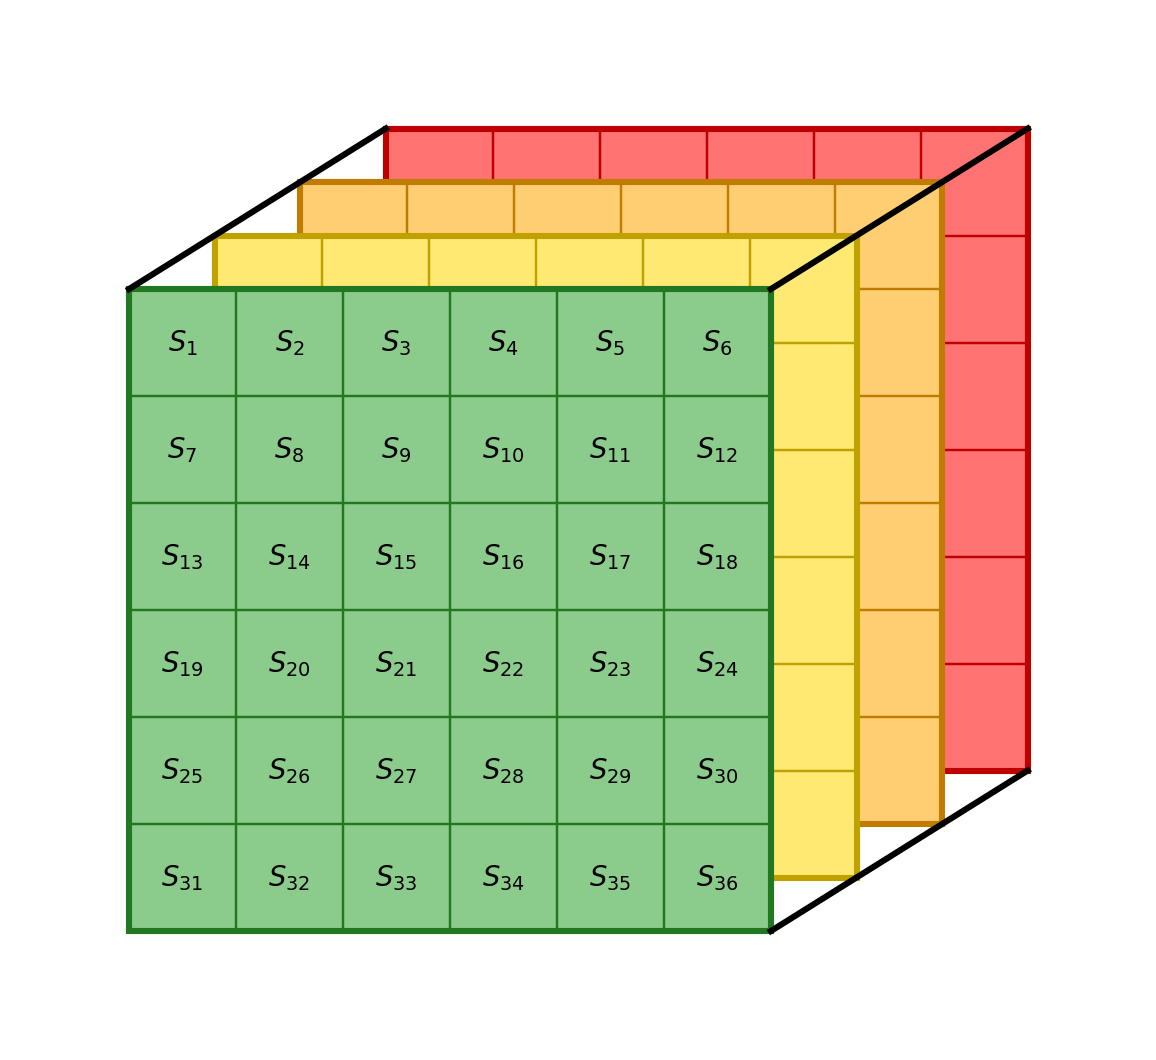
\includegraphics[width=0.575\textwidth]{immagini/spot_cubo.png}
	\caption{Rappresentazione spots e geni}
	\label{fig:four}
\end{figure}

La figura ~\ref{fig:four} mostra una rappresentazione grafica degli spot e dei geni all'interno di un tessuto. Ogni cella rappresenta uno spot, mentre ogni colore rappresenta un gene diverso\footnote{Si noti che il colore non è rappresentativo della presenza o meno di quel gene in quello spot}.
Si può notare che ogni spot $\mathbb{S}_i$, al suo interno, può contenere più geni.
Inoltre, nella figura d'esempio, si hanno 36 spot diversi e 4 geni, ma ma nella realtà i dati
sono differenti: gli spot possono arrivare a oltre 3000
celle e i geni possono superare i 30,000.

La figura \ref{fig:four}, tuttavia, presenta una inesattezza in quanto gli spot non sono disposti su una matrice $n \times n$, bensì hanno una rappresentazione esagonale.
Questo significa che, dato uno spot $\mathbb{S}_i$, questo presenterà sei spot
adiacenti, tranne nei casi in cui gli spot sono localizzati ai bordi del tessuto.

Per poter trovare spazialmente uno spot $\mathbb{S}_i$, quindi, occorre assegnare una coordinata $x$ e una coordinata $y$ ad ogni spot, e, una volta creata una matrice \\$[\mathbb{S}_i, <x_i, y_i>]$,
dove $<x, y>$ indicano le coordinate dello spot, è possibile trovare i 6 vicini attraverso un semplice calcolo.
Inoltre, per sopperire ad eventuali spazi vuoti nel tessuto, viene calcolata la distanza euclidea tra gli spot, in modo da poter scartare gli spot che altrimenti verrebbero erronamente segnati come vicini.

La figura~\ref{fig:five} mostra una rappresentazione grafica degli spot in un tessuto, con le loro coordinate $x$ e $y$.
Lo spot preso in esempio, come riferimento, è lo spot con coordinate $x = 2, y = 3$.
\begin{figure}[ht]
	\centering
	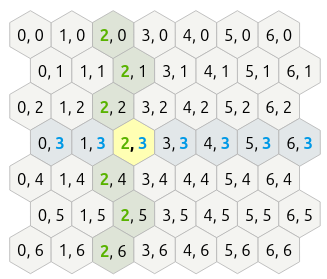
\includegraphics[width=0.5\textwidth]{immagini/spotRappresentazioneEsagonale.png}
	\caption{Rappresentazione spaziale spots}
	\label{fig:five}
\end{figure}

\section{Smoothing spaziale}\label{sec:cap_two_notions}
Quando si entra in possesso di una library, contenente i barcode degli spot, le coordinate spaziali e i relativi metadati, non è consigliato
avviare l'analisi dei dati fin da subito, 
questo perchè i dati di TS contengono anche rumore tecnico e biologico che può mascherare dei pattern in realtà utili, come ad esempio dei geni con profili irregolari.
Occorre quindi prima di tutto ripulire e ridurre la complessità dei dati prima di poterli analizzare.

\medskip
Uno dei primi step per poter poter minimizzare il rumore è applicare un \textit{filtro di media} (Mean Filter),
ovvero una tecnica per poter sostituire ogni elemento, con la media dei valori dei suoi vicini dato un raggio prestabilito\cite{Giotto}.
Questo serve per poter ridurre il rumore locale ed evitare variazioni importanti.

Considerando un tessuto a due dimensioni, contenente $\mathbb{S}$ spots e $\mathbb{G}$ geni.
Possiamo denotare con $y_{ij} \in \mathbb{R}$ il livello di espressione genica di un determinato gene $g_i$ nello spot $\mathbb{S}_i$.
Dalla definizione di matrice di espressione genica $X$ definita precedentemente, possiamo ora definire $\widehat{X}$ la matrice ottenuta come output 
dopo aver applicato la seguente operazione:
\begin{equation}
\hat y_{ij} = \sum_{s_k \in \mathcal{N}_r(s_j)} w_{jk} \cdot y_{ik}
\label{eq:smoothing}
\end{equation}
dove $N_r(s_j) = \{ s_k \mid \| s_k - s_j \| \le r,\; s_k \in \mathbb{S} \}$ con raggio $r \in \mathbb{R}$ denota i vicini dello spot $s_j$, e $w_{jk}$ sono i pesi spaziali 
che soddisfano $\sum_k w_{jk} = 1$.

Per trovare i pesi spaziali poi, viene applicato il filtro di media:
\begin{equation}
	w_{jk} = \frac{1}{\mid \mathcal{N}_r(s_j)\mid}
\label{eq:filtroDiMedia}
\end{equation}
dove $\mathcal{N}_r(s_j)$ denota i vicini dello spot $s_j$ entro il raggio $r$, e tutti i vicini contribuiscono in modo equivalente.

\medskip
\noindent
In alternativa al filtro di media è possibile utilizzare la \textit{Gaussian Kernel Smoothing}\cite{GaussianKernelSmoothing} per calcololare i pesi spaziali.
Prima si devono calcolare i pesi non normalizzati usando un Kernel Gaussiano:
\begin{equation}
	\widetilde w_{jk} = \frac{1}{\sigma\sqrt{2\pi}}\,
\exp\!\left(-\,\frac{\lVert s_k - s_j\rVert^{2}}{2\sigma^{2}}\right)
\label{eq:gaussianKernel}
\end{equation}
dove $\sigma$ controlla la portata spaziale di smoothing.
Dopodichè andremo ad applicare una normalizzazione\footnote{Dividere tutti i termini di un'espressione per uno stesso fattore in modo che l'espressione risultante abbia una certa norma uguale a 1.} per ottenere i pesi finali:
\begin{equation}
	w_{jk} = \frac{\widetilde{w}_{jk}}{\sum_h \widetilde{w}_{jh}}
\label{eq:gaussianKernelNormalization}
\end{equation}
garantendo che $\sum_k w_{jk} = 1$ per ogni spot $s_j$.

\begin{figure}[ht]
	\centering
	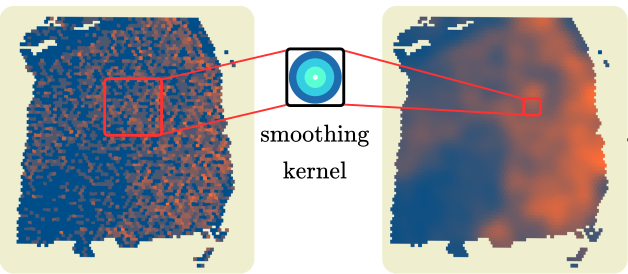
\includegraphics[width=0.8\textwidth]{immagini/spatialSmoothing.png}
	\caption{Dimostrazione di Smoothing Spaziale}
	\label{fig:six}
\end{figure}

La figura \ref{fig:six} dimostra come filtro di media attenua le variazioni locali, riducendo i valori e producendo una mappa più omogenea dove i picchi isolati di rumore risultano smussati.


\medskip
\noindent
\paragraph{Smoothing Spaziale a due fattori}
Un'altra variante allo smoothing visto sopra è lo \textit{smoothing a due fattori}, che combina i vicini spaziali e la loro somiglianza trascrizionale, ovvero i pattern.
Usando lo smoothing a due fattori, i dati smussati risultano essere più accurati nelle loro partizioni e interpretazioni biologiche rispetto all'utilizzo di operazioni a un fattore\cite{smoothingTwoFactors}.

Dato $\mathcal{X}_i$ un vettore di espressione genica per uno spot $i$, 
la sua versione smussata $\mathcal{X}_i'$ può essere calcolata come segue:

\begin{equation}
\mathcal{X}_{i}' = (1-\alpha)\,\mathcal{X}_{i} + \alpha \left(
    \beta \frac{\sum_{j \in {N}_s(i)} c^{s}_{ji}\,\mathcal{X}_{j}}
               {\sum_{k \in {N}_s(i)}\, c_{ki}^s}
    + (1-\beta) \frac{\sum_{j \in {N}_p(i)} c^{p}_{ji}\,\mathcal{X}_{j}}
                      {\sum_{k \in {N}_p(i)}\, c_{ki}^p}
\right).
\label{eq:smoothingTwoFactors}
\end{equation}
Nella equazione \ref{eq:smoothingTwoFactors} ci sono due parametri, $\alpha$ e $\beta$.
La prima  regolarizza il rapporto tra l'espressione originale e quella corretta, 
evitando che l'espressione dello spot in esame risulti eccessivamente smussata.
$\beta$ invece modula il peso relativo dello smussamento basato sulla vicinanza spaziale rispetto a quello basato sui pattern.
$N_s(i)$ e $N_p(i)$ indicano, rispettivamente, i vicini spaziali e i pattern nello spot $i$.
$c^{p}_{ji}$ e $c^{s}_{ji}$ indicano, rispettivamente, il contributo spaziale e quello di pattern dello spot $j$ vicino allo spot in oggetto $i$.
\section{Formato dei dati}\label{sec:cap_three_notions}
I dati del campione di tessuto fornitoci sono in formato \textit{10x Visium}, una piattaforma 
di trascrittomica spaziale che misura l'espressione genica 
su sezioni di tessuto, mantenendo per ogni misura la posizione spaziale. 
La cattura avviene su spot barcodati stampati su una slide. Il programma che processa i dati in modo da mappare i barcode con la loro 
posizione spaziale viene chiamato \textit{Space Ranger} e produce la matrice \textit{Features}$\times$\textit{Barcodes}, dove con Features si intendono i geni, 
e con Barcodes i vari spot; 
Ogni spot raccoglie RNA da più cellule e i conteggi vengono poi mappati sull'immagine.


I file 10x Visium sono in formato \texttt{.h5}, un file specifico pronto per essere elaborato da \texttt{ScanPy} una libreria Python\footnote{Linguaggio di programmazione di alto livello, interpretato e open source}
open-source\footnote{Codice sorgente libero} progettata per l'analisi di dati di trascrittomica.
Scanpy infatti offre la funzione \texttt{sc.read\_visium()} per importare direttamente le cartelle di output di Space Ranger.

Prendendo il file \texttt{.h5} e traducendolo in un file \texttt{.tsv} (Tab-Separated Values) si può osservare una struttura di questo tipo:
\begin{table}[H]
\centering
\caption{Estratto metadati spot (dataset \texttt{1.DLPFC}).}
\label{tab:tsvTable}
\resizebox{\textwidth}{!}{%
\begin{tabular}{lcccc}
\hline
\textbf{Barcode} & \textbf{Row} & \textbf{Col} & \textbf{Cluster} & \textbf{sum\_Gene} \\
\hline
AAACAAGTATCTCCCA-1 & 1 & 3 & 7 & 3586 \\
AAACAATCTACTAGCA-1 & 1 & 27  & 4 & 1150 \\
AAACACCAATAACTGC-1 & 1 & 59 & 8 & 1960 \\
\hline
\end{tabular}%
}
\end{table}
\begin{minipage}{\textwidth}
\centering
\label{tab:legendTsvTable}
\footnotesize
\texttt{barcode}: identificatore dello spot;\;
\texttt{sample\_name}: nome del campione;\;\\
\texttt{row}, \texttt{col}: coordinate dello spot nella griglia;\;\\
\texttt{Cluster}: cluster di appartenenza;\;
\texttt{sum\_gene}: numero totale di geni rilevati.
\end{minipage}

La tabella \ref{tab:tsvTable} è solo una sezione di cosa contiene davvero il file \texttt{.h5}, nella realtà sono presenti svariagi gigabyte di dati.

Oltre ai file sopracitati viene fornita anche una cartella chiama \texttt{spatial} contenente immagini ad alta e bassa definizione 
del tessuto, e il file delle posizioni degli spot chiamato \texttt{tissue\_positions.csv}

\begin{figure}[ht]
	\centering
	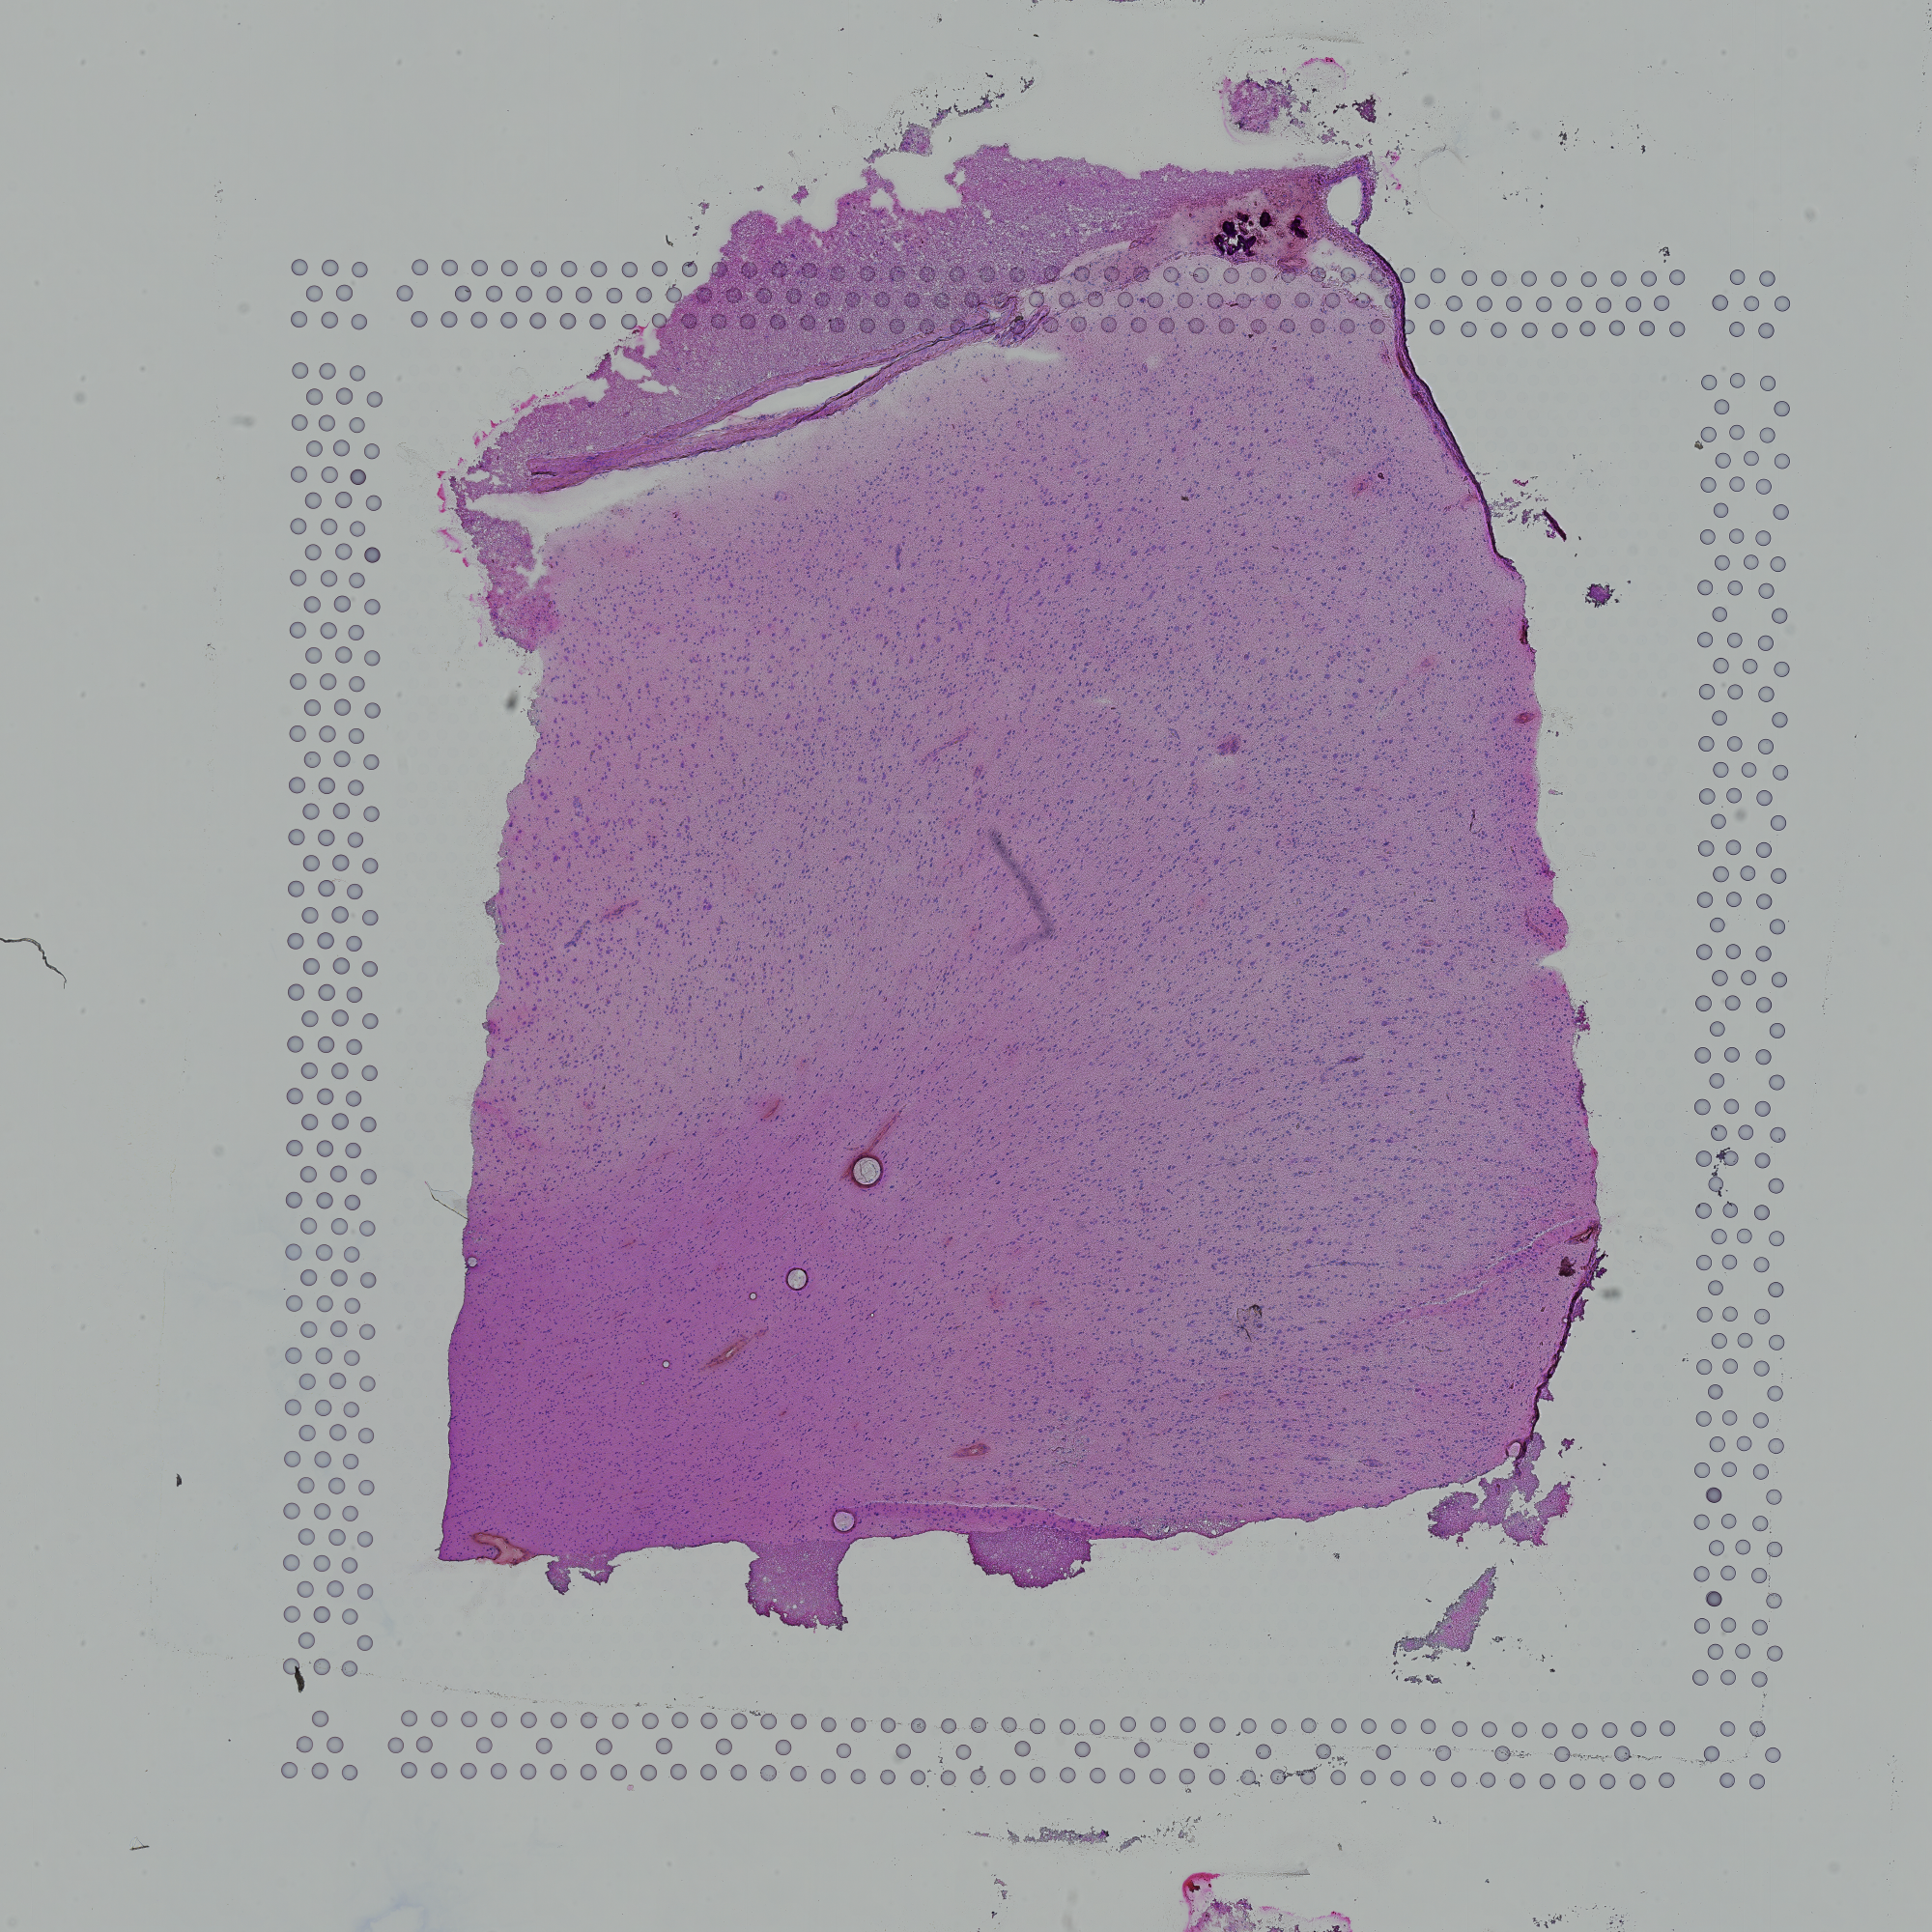
\includegraphics[width=0.8\textwidth]{immagini/tissue_hires_image.png}
	\caption{File che contiene la foto del tessuto: \texttt{tissue\_hires\_image.png}}
	\label{fig:seven}
\end{figure}

\section{Scanpy}\label{sec:cap_four_notions}
Scanpy è un toolkit in Python per l'analisi di dati di espressione genica a singola cellula, 
progettato per lavorare anche con dataset molto estesi e per integrarsi con l'ecosistema Python. 
Include metodi per il pre-processing, come filtri su cellule e geni, normalizzazione, identificazione degli HVGs e clustering. 

Scanpy fornisce inoltre funzioni con velocità elevate che rendono l'analisi di 
data set con più di un milione di cellule e interrogazioni real time nell'ordine di secondi per data set con circa 100,000 cellule.
Questa moltitudine di funzioni, assieme ad velocità non indifferente, ne hanno favorito l'adozione in molti ambiti di ricerca.\cite{scanPyUsage}

Dal punto di vista della manutenibilità invece, Scanpy è sviluppato nell'mbito del progetto \textit{scverse}, 
che coordina strumenti fondamentali per l'analisi omica in Python. 
Questo garantisce linee guida comuni, interoperabilità tra pacchetti e una documentazione unificata, 
elementi cruciali in contesti accademici e clinici dove la tracciabilità delle analisi è essenziale.\cite{scverse}

\medskip
\noindent
Le funzioni della libreria sono organizzate per famiglie:
\begin{itemize}
	\item \texttt{sc.pp.*} rigurda le varie funzioni per il pre-processing.
	\item \texttt{sc.tl.*} serve per gli strumenti analitici, come clustering o creazione di grafi.
	\item \texttt{sc.pl.*} infine riguarda le varie funzioni usate per la visualizzazione, con cui è possibile stampare a video delle immagini.
\end{itemize}

\noindent
Per la trascrittomica spaziale, 
Scanpy offre un'integrazione naturale con i dati 10x Visium tramite 
\texttt{scanpy.read\_visium()}, che carica non solo la matrice di espressione ma anche immagini e coordinate degli spot. 
La funzione ha la seguente firma:

\begin{center}
\begin{minipage}{8cm}
\begin{verbatim}
scanpy.read_visium(
    path,
    genome = None,
    count_file = 'filtered_feature_bc_matrix.h5',
    library_id = None,
    load_images = True,
    source_image_path = None
	)
\end{verbatim}
\end{minipage}
\end{center}

\noindent
Gli argomenti della funzione sono i seguenti:
\begin{itemize}
  \item \texttt{path}: Percorso alla cartella radice che contiene l'output Visium, ovvero il file \texttt{.h5} e la sottocartella \texttt{spatial/}.
  \item \texttt{genome}: Opzionale, è lidentificatore del genoma che si vuole filtrare, se presente nei metadati 10x.
  \item \texttt{count\_file}: Nome del file di 10x Visium contenente i vari dati. Deve essere presente nella cartella inserita in \texttt{path}. Di default ha come nome (\texttt{filtered\_feature\_bc\_matrix.h5} per default.
  \item \texttt{library\_id}: Opzionale, e l'dentificativo della libreria Visium. Risulta utile quando occorre concatenare più librerie.
  \item \texttt{load\_images}: Se \texttt{True}, carica le immagini del tessuto.
  \item \texttt{source\_image\_path}: Opzionale, è il percorso alternativo da cui leggere le immagini se non si trovano in \texttt{spatial/}.
\end{itemize}

\noindent
La funzione restituisce un oggetto \texttt{AnnData}, una struttura dati che accoppia in modo coerente la matrice di espressione con annotazioni su spot 
e geni, oltre che a campi dedicati per grafi e metadati.
\texttt{anndata.X} contiene la matrice \textit{Features}$\times$\textit{Barcodes}, \texttt{anndata.obs} da \textit{Observations} contiene tutti e solo i barcodes degli spot, mentre 
\texttt{anndata.vars} da \textit{Variables} contiene tutti e solo i geni misurati, con nome, id e tipo.
Gli oggetti \texttt{AnnData} si possono salvare tramite la funzione \texttt{anndata.write\_h5ad()} e i file così creati hanno estensione \texttt{.h5ad}.

\medskip
\noindent
La funzione sopracitata ha la seguente firma:
\begin{center}
\begin{minipage}{8cm}
\begin{verbatim}
anndata.write_h5ad(
		filename,
		compression = hdf5plugin.FILTERS["zstd"]
	)
\end{verbatim}
\end{minipage}
\end{center}

\noindent
Con come argomenti: 
\begin{itemize}
  \item \texttt{filename}: Il nome del file che si vuole salvare con estensione \texttt{.h5ad}.
  \item \texttt{compression}: Opzionale, metodi alternativi di compressione del file.
 \end{itemize}

Un esempio completo di un programma scritto in linguaggio Python con lettura dei dati 10x Visium attraverso Scanpy e 
relativo salvataggio di AnnData in formato \texttt{.h5ad} è il seguente:

\begin{lstlisting}[style=mypython, caption={Funzione per caricare il file \texttt{.h5} ed esempio su come utilizzarla per inizializzare oggetto \texttt{AnnData}}]
import scanpy as sc

def load_data():
    
    adata_gene_expression = sc.read_visium("1.DLPFC/151673", count_file="filtered_feature_bc_matrix.h5", load_images=True)
    
    return adata_gene_expression

annData = load_data()

annData.write_h5ad(filename="processed_adata")
\end{lstlisting}

\section{Ottenimento Maschere Binarie dei geni}\label{cap:BinaryMasks}
Una volta ottenuti i dati in formato \texttt{AnnData} è possibile iniziare a manipolarli come oggetto per poterne ricavare le varie informazioni 
necessarie allo studio che si sta svolgendo.

Come detto in precendeza occorre applicare prima di tutto uno Smoothing per poter ripulire e ridurre la complessità dei dati ottenuti.
Questo smoothing viene applicato gene per gene attraverso il filtro di media, definito precedentemente, in questo modo:
\begin{lstlisting}[style=mypython,label=code:MeanFilter,caption={Funzioni per ottenere i dati di un gene specifico e applicarci il filtro di media}]
	ITNI = np.zeros((nspot, 7), dtype=int)
	VNI   = (ITNI!=-1).astype(int)
    NN    = VNI.sum(axis=1)
    NM    = (VNI.T / NN.T).T

	def get_gene_data(data, gene_id):
		array_data = data.X.toarray().T
		gene_data  = array_data[gene_id]
		return gene_data
	
	def super_opt_mean_filter(gene_data):
		global ITNI, NM
		return (gene_data[ITNI] * NM).sum(axis=1)

	def opt_mean_filter_iterated(gene_data, it):
		for _ in range(it):
			gene_data = super_opt_mean_filter(gene_data)
		return gene_data
	
	geneData = get_gene_data(anndata, 1)

	geneData = opt_mean_filter_iterated(gdata, 5)
\end{lstlisting}

Lo Snippet del codice \ref{code:MeanFilter} presenta 3 funzioni principali che permettono di utilizzare il filtro di media: la prima, 
\texttt{get\_gene\_data(data, gene\_id)}, permette di recuperare dall'oggetto \texttt{AnnData} un gene dato il suo \texttt{id}.
Il suo funzionamento è molto basico in quanto intuitivamente viene creata una variabile contenente la matrice trasposta di \texttt{AnnData.X}, che, come detto precedentemente, l'oggetto \texttt{X} 
all'interno di \texttt{AnnData} contiene la matrice \textit{Features}$\times$\textit{Barcodes}, e rendendola trasposta essa viene trasformata in \textit{Barcodes}$\times$\textit{Features}, ovvero anzichè avere 
in ogni riga uno spot e per ogni colonna l'espressione genica di un determinato gene su quello spot, si otterrà invece un gene per ogni riga, e la sua espressione genica su ogni spot per ogni colonna.
La tabella \ref{tab:ann_data_and_transpose} contiene una rappresentazione visiva della matrcie \texttt{AnnData.X} e della sua relativa trasposta.

\begin{table}[htbp]
  \centering
  \caption{Struttura di \texttt{AnnData.X} e della sua trasposta}
  \label{tab:ann_data_and_transpose}
  
  \textbf{Matrice $X = \texttt{AnnData.X}$} \\[0.5em]
  \begin{tabular}{c|ccc}
    & Gene1 & Gene2 & Gene3 \\
    \hline
    Spot1 & $0$ & $10$ & $24$ \\
    Spot2 & $15$ & $2$ & $0$ \\
    Spot3 & $14$ & $12$ & $23$ \\
  \end{tabular}

  \vspace{2em} 

  \textbf{Trasposta $X^\top$} \\[0.5em]
  \begin{tabular}{c|ccc}
    & Spot1 & Spot2 & Spot3 \\
    \hline
    Gene1 & $0$ & $15$ & $14$ \\
    Gene2 & $10$ & $2$ & $12$ \\
    Gene3 & $24$ & $0$ & $23$ \\
  \end{tabular}
  
\end{table}


La seconda funzione, \texttt{super\_opt\_mean\_filter(gene\_data)}, implementa un filtro di media sui valori di espressione genica sfruttando operazioni completamente vettorizzate.
Prima della funzione vengono definite alcune variabili di supporto:

\begin{itemize}
\item \texttt{ITNI}: matrice di forma $(n_{spot}, 7)$ contenente, per ogni spot, gli indici dei suoi vicini. Gli elementi pari a \texttt{-1} indicano assenza di vicino.
\item \texttt{VNI = (ITNI != -1)}: maschera binaria che vale $1$ dove l'indice è valido e $0$ altrimenti.
\item \texttt{NN = VNI.sum(axis=1)}: numero di vicini validi per ciascuno spot.
\item \texttt{NM = (VNI.T / NN.T).T}: matrice di pesi normalizzati, dove ogni vicino valido riceve un peso pari a $\frac{1}{NN_i}$.
\end{itemize}

La funzione calcola la media dei valori di espressione di un gene sui vicini di ciascuno spot.
Ogni riga della matrice \texttt{gene\_data[ITNI]} contiene i valori del gene nei vicini di uno spot, che vengono moltiplicati per i pesi corrispondenti in \texttt{NM} e poi sommati.
Il risultato è un vettore in cui ogni elemento rappresenta la media dei valori di espressione nei vicini.

La terza funzione, \texttt{opt\_mean\_filter\_iterated(gene\_data, it)}, semplicemente itera \texttt{it} volte la funzione precedente.
Questo perchè iterando più volte il filtro di media, ottengo una rappresentazione più accurata del valore dei vicini di ogni gene, e quindi ottenendo una rappresentazione migliore delle zone più dense.
\newline

\begin{figure}[ht]
	\centering
	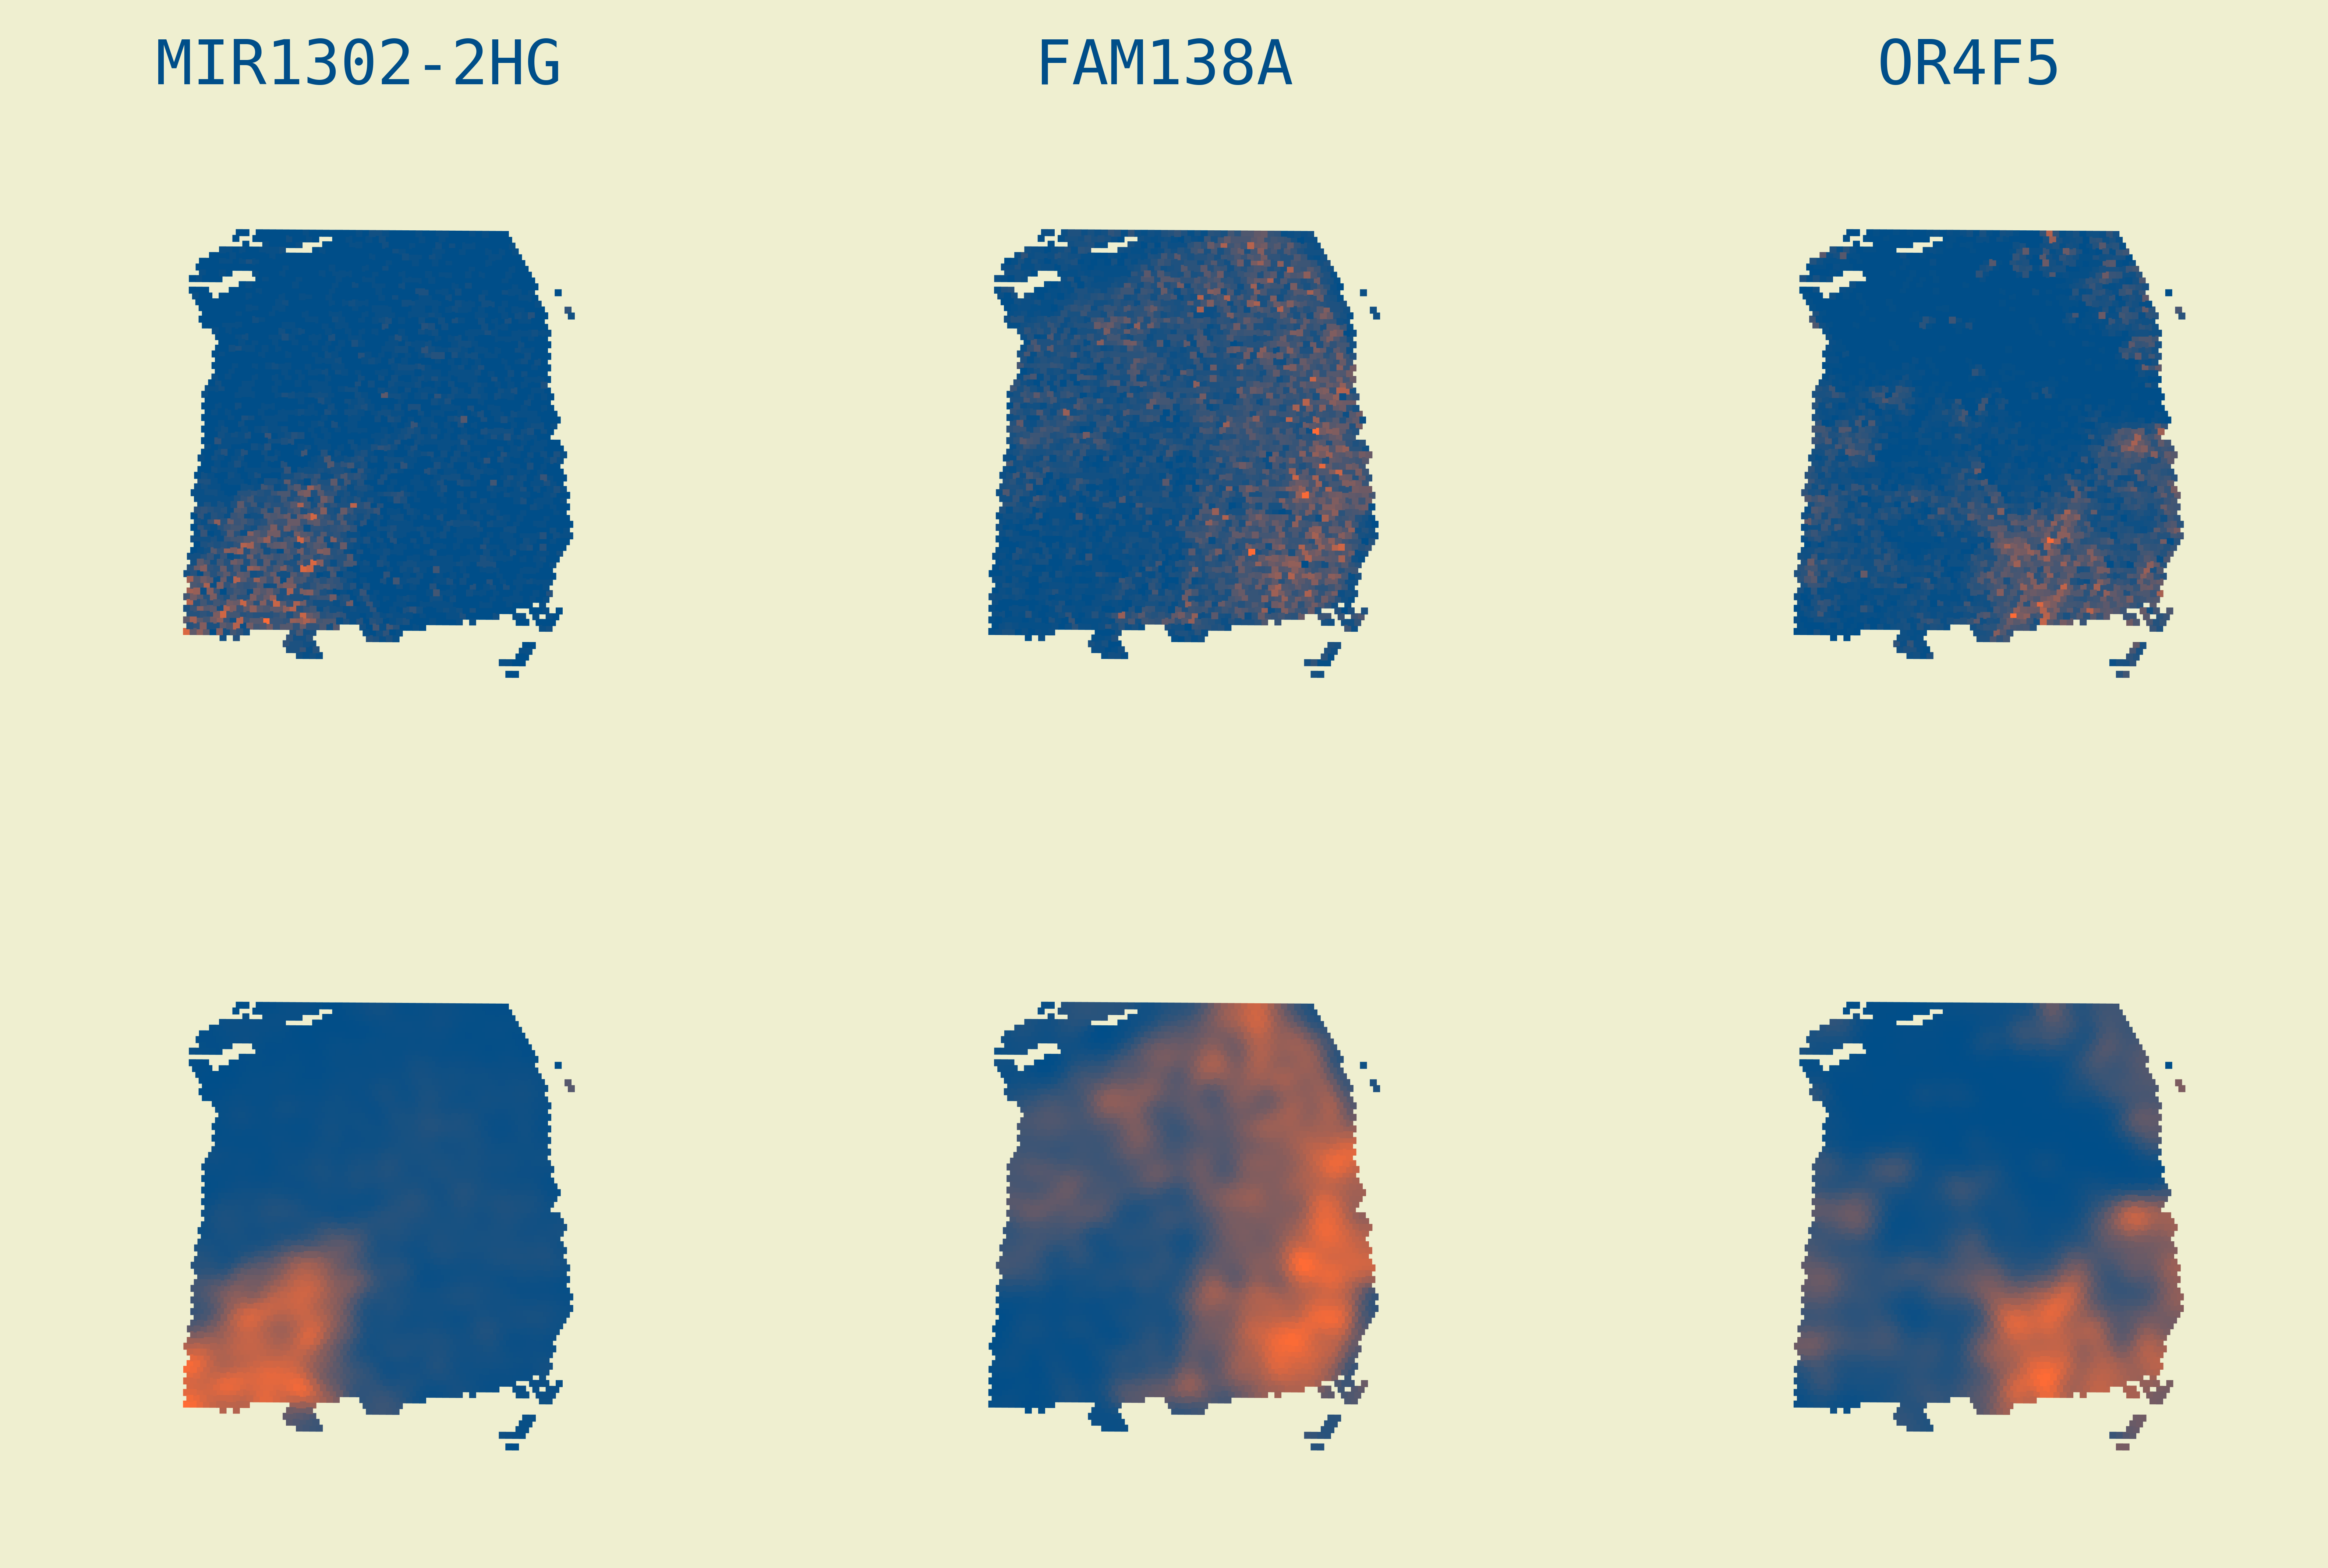
\includegraphics[width=0.8\textwidth]{immagini/mean_filter.png}
	\caption{Rappresentazione di alcuni geni prima e dopo il filtro di media}
	\label{fig:meanFilter}
\end{figure}

Una volta ottenuto i vari geni con le loro espressioni geniche "smussate" dal filtro di media, stimiamo per ogni gene 
un modello di misura  $\forall k \text{ tale che } 1 \le k \le 10$ gaussiane, attraverso la funzione di \texttt{sklearn.mixture.GaussianMixture()}.
Questo algoritmo cerca di adattare, per ciascun valore di $k$, 
una combinazione\footnote{In inglese: mixture} di $k$ distribuzioni gaussiane 
ai dati di espressione del gene in esame, al fine di modellare la presenza di sottopopolazioni 
o modalità multiple nell'espressione. 

\begin{figure}[ht]
	\centering
	
\includegraphics[width=1\textwidth]{immagini/gauss_misxture_multik.png}
	\caption{Dimostrazione di come diverse $k$ rappresentano diversamente i dati}
	\label{fig:gaussianMixture}
\end{figure}

Si può osservare dalla figura \ref{fig:gaussianMixture} come con $1 \le k$ la rappresentazione non colga efficacemente ogni picco dell'espressione genica del gene preso in esame; Si verifica perciò un fenomeno di \textit{underfitting}\footnote{Modello troppo semplice per catturare la complessità dei dati}.
Al contario, con $k \> 3$ si verifica il problema opposto, ovvero ho troppe gaussiane per rappresentare efficacemente i dati in oggetto, si verifica perciò dell'\textit{overfitting}.
Nell'esempio della figura \ref{fig:gaussianMixture} perciò la $k$ corretta corrisponde a $k = 3$.

Per poter scegliere in autonomia la $k$ corretta, 
una volta allenata la funzione \texttt{sklearn.mixture.GaussianMixture()} con un gene, 
si salva attraverso la funzione \texttt{GaussianMixture().bic()} il \textit{Bayesian Information Criterion}(BIC) corrispondente a tale $k$ su quel gene.
Il BIC è un indice statistico che misura quanto bene un modello spiega i dati passati, 
penalizzando i modelli troppo complessi.

La formula con la quale si può ottenere è la seguente:
\begin{equation}
	\mathrm{BIC} = k \cdot \ln(n) - 2 \cdot \ln(\widehat{L})
\end{equation}
dove $n$ indica il numero degli spots, $k$ il numero di parametri stimati dal modello, $\widehat{L}$ massima verosimiglianza del modello, 
ovvero quanto bene il modello si adatta ai dati.

Una volta ottenuti i vari BIC per ogni $k$, viene infine scelta la $k$ corretta attraverso il calcolo del "Knee Point".
Il Knee Point, altro non è che il punto in cui la curva cambia inclinazione in modo evidente, 
passando da una salita marcata a una più piatta, o viceversa.

\begin{figure}[ht]
	\centering
	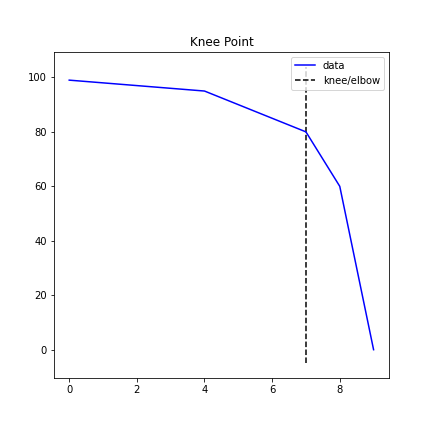
\includegraphics[width=0.6\textwidth]{immagini/kneeOfACurve.png}
	\caption{Esempio di Knee Point}
	\label{fig:kneePoint}
\end{figure}

\noindent
Il codice Python per poter calcolare relativi BIC e Knee Point è il seguente:

\begin{lstlisting}[style=mypython,label=code:gmmAndKnee,caption={Funzioni per ottenere BIC e KP}]
	def gmm_BIC(gdata, mink=2, maxk=10):

		data = gdata.reshape(-1, 1)
		bics = []

		for i in range(mink, maxk+1):
			gmm = GaussianMixture(n_components=i, 
								  random_state=0)
								  	.fit(data)
			BIC_gmm = gmm.bic(data)
			bics.append(BIC_gmm)

		return bics
	
	def find_knee(x, y):
		knee_locator = kneed
						.KneeLocator(
							x, 
							y, 
					 		interp_method="polynomial", 
							curve="convex", 
							direction="decreasing")
		knee   = knee_locator.knee  
			
		return knee
	
	mink = 1
	maxk = 10
	x    = np.arange(mink, maxk+1)
	
	bics = gmm_BIC(gdata, mink, maxk)
	k    = find_knee(x, bics, plt.gca())
\end{lstlisting}

Una volta ottenuta la $k$ ottimale tramite il Knee Point, si può creare la
maschera binaria per il gene in esame. 
La maschera binaria identifica, per ogni spot, se il gene è espresso (1) oppure no (0), 
in base alla soglia determinata dal modello Gaussian Mixture.
Il procedimento è il seguente:
\begin{enumerate}
	\item Si allena il modello GaussianMixture con $k$ componenti sul vettore di espressione genica smussato.
	\item Si assegna ogni spot alla componente gaussiana con la media più alta, presenza del gene, oppure più bassa, assenza.
	\item Si crea la maschera binaria: 1 se lo spot appartiene alla componente con media maggiore, 0 altrimenti.
\end{enumerate}

Questo procedimento mi porterà ad avere un array, di lunghezza \texttt{len($n_{\text{spots}}$)} in cui avrò valore 1 se il gene risulta presente nello spot $s_i$, oppure 0,  con $1 \le i \le s_n$.
\newpage
Il codice per generare la maschera binaria è il seguente:
\begin{lstlisting}[style=mypython,label=code:binaryMask,caption={Funzioni per ottenere le machere binarie una volta ottenuta la k del Knee Point}]
	def fit_MoG(gdata, k):
		data = gdata.reshape(-1, 1)
		gmm  = GaussianMixture(n_components=k,
							   random_state=0)
							   		.fit(data)
		mus  = gmm.means_
		stds = np.sqrt(gmm.covariances_)
		return mus, stds

	def smallest_dist(mus, stds):
    	idx = np.argmin(mus)
    	return mus[idx][0], stds[idx][0][0]
	
	def expansion_filter(gene_data):
		global ITSNI, HNN
		active_neigh = gene_data[ITSNI].sum(axis=1)
		return (active_neigh >= 3)
					.astype(int) * 
					 gene_data + 
					 (active_neigh > 3)
						.astype(int) * 
						 (1-gene_data)

	def expansion_filter_iterated(gene_data, it):
		for _ in range(it):
			gene_data = expansion_filter(gene_data)
		return gene_data
	
	ITSNI = ITNI[:,1:]
    HNN   = NN//2
	mus, stds = fit_MoG(gdata, k)
    m, v = smallest_dist(mus, stds)
    pgdata = expansion_filter_iterated((gdata>(m+1.5*v))
									  	.astype(int), 10)
\end{lstlisting}


Segue la spiegazione di quanto avviene nel codice \ref{code:binaryMask}:

\begin{itemize}
	\item La funzione \texttt{fit\_MoG()} riceve il vettore di espressione smussata \texttt{gdata} e il numero di componenti $k$ trovate dal Knee Point. Viene poi trasformata in colonna da \texttt{gdata.reshape(-1,1)} per adattarsi al modello GaussianMixture. Il modello viene addestrato e restituisce i vettori di medie \texttt{mus} e deviazioni standard \texttt{stds} delle gaussiane. 
  	\item \texttt{smallest\_dist} seleziona la gaussiana con la media più bassa, salvandola nell'indice \texttt{idx}, assumendo che quella rappresenti l'assenza di espressione. Restituisce poi la media $m$ e la deviazione standard $v$ di quella componente.
	\item Nella codice \texttt{gdata > (m + 1.5 * v)).\text{astype(int)}} passato come argomento alla funzione \texttt{expansion\_filter\_iterated}
		si applica la soglia $m + 1.5\cdot v$ per trasformare i valori continui in una prima maschera binaria grezza: gli spot con espressione maggiore rispetto a quella soglia sono considerati attivi, $1$, altrimenti inattivi, $0$.
	\item \texttt{expansion\_filter} raffina questa maschera binaria guardando i vicini: 
		\begin{itemize}
			\item Si calcola il numero di vicini attivi per ciascun spot (\texttt{active\_neigh}).  
			\item Se un vicino ha almeno 3 vicini attivi, si mantiene il valore attuale (\(\texttt{* gene\_data}\)).  
			\item Se ha più di 3 vicini attivi, si può invertire il valore dello spot (\(1 - \texttt{gene\_data}\)) per favorire l'espansione del segnale.
		\end{itemize}
	\item \texttt{expansion\_filter\_iterated} applica iterativamente il filtro per \texttt{it} cicli, permettendo al pattern attivo di “espandersi” su regioni contigue.
	\item Infine, la variabile \texttt{pgdata} contiene la maschera binaria finale raffinata: si parte da una soglia basata sulla componente con media minima, poi si enfatizza la coerenza spaziale tramite l'espansione iterata $10$ volte.
\end{itemize}

\begin{figure}[ht]
	\centering
	
\includegraphics[width=0.8\textwidth]{immagini/transf_ex3.png}
	\caption{Gene da dati iniziali a maschera binaria}
	\label{fig:fromRawToBinaryMask}
\end{figure}
% !TeX spellcheck = it_IT
\chapter{Sviluppo e risultati sperimentali}\label{chapter:MineStuff}
Dopo aver presentato nel Capitolo precedente le nozioni 
fondamentali e le operazioni di pre-processing necessarie 
alla gestione dei dati, in questo capitolo 
verrà descritto lo sviluppo pratico e le analisi sperimentale svolta.  
L'obiettivo principale è quello di progettare e realizzare 
una metodologia computazionale in grado di 
identificare \textit{clustering alternativi} nei dati di trascrittomica spaziale, 
fornendo una rappresentazione più flessibile e interpretabile dei 
domini genici rispetto agli approcci convenzionali.

Per fare ciò è necessario che ogni gene venga e suddiviso spazialmente in sottogeni, affinchè essi si possano 
catalogare tra di loro e poter analizzare eventuali relazioni particolari che ci sono fra un sottogene e un altro.
\section{Grafo dei vicini}\label{subsec:Vicini}
Come prima cosa, come mostrato nella figura \ref{fig:five}, è necessario individuare per ogni spot $s_i$ 
l'insieme dei suoi spot adiacenti, ovvero la lista dei \textit{vicini}. 
Questa informazione è fondamentale poiché consente di stabilire quando due geni si trovano in prossimità spaziale,
condizione necessaria per poter poi definire relazioni di vicinanza, contiguità e sovrapposizione tra geni attivi.

I dati forniti dalla tecnologia 10x Visium contengono, per ciascuno spot, 
le sue coordinate sulla griglia di cattura. 
Tuttavia, tali coordinate sono organizzate in forma tabellare, come visto nella tabella \ref{tab:tsvTable}, all'interno della struttura \texttt{scdata.obs},
e perciò non immediatamente interpretabili in termini spaziali. 
Per poter costruire un grafo dei vicini è quindi necessario effettuare una conversione preliminare di queste informazioni,
trasformando le coordinate della griglia in coordinate cartesiane.
In questo modo è possibile rappresentare ogni spot come un punto nel piano, preservando le distanze e la disposizione
esagonale della griglia Visium.

\begin{lstlisting}[style=mypython,
                   label=code:index_to_cart,
                   caption={Trasformazione delle coordinate spaziali in coordinate cartesiane}]
    index_to_cart = np.zeros((len(scdata.obs), 2))
    max_row       = scdata.obs['array_row'].max()
    for i, ind in enumerate(scdata.obs.index):
        col = scdata.obs['array_col'][ind]
        row = scdata.obs['array_row'][ind]
        index_to_cart[i, 0] = col * (np.sqrt(3)/2)
        index_to_cart[i, 1] = (max_row - row) * (3/2)
\end{lstlisting}


Il frammento di codice \ref{code:index_to_cart} mostra come vengono calcolate e salvate le coordinate cartesiane di ciascuno spot,
partendo dalle colonne \texttt{array\_row} e \texttt{array\_col} della tabella di input. 
Viene inoltre applicata una correzione di scala per tenere conto della disposizione esagonale della griglia,
in cui le colonne sono sfalsate e le distanze orizzontali e verticali non sono equivalenti.

\paragraph{Costruzione del grafo dei vicini con k\text{-}NN.}
Definite le coordinate cartesiane $\mathbb{R}^2$ per ciascuno spot, 
il passo successivo consiste nell'identificare, per ogni spot $s_i$ 
i sei spot più prossimi nella griglia esagonale 10x Visium. 
A tal fine è stato impiegato l'algoritmo dei \textit{Nearest Neighbors} (k\text{-}NN), 
nella sua implementazione fornita dalla libreria \texttt{sklearn.neighbors}, 
libreria che implementa la funzione (\texttt{NearestNeighbors( ... )}).
L'idea dietro la funzione è la seguente: dato l'insieme di punti $\{x_1, ..., x_n\} \in \mathbb{R}^2$, 
per ciascun punto $\mathbf{x}_i$ si ricercano i $k$ vicini
più prossimi secondo una metrica prefissata, come la distanza euclidea. 
Poiché la funzione restituisce anche il punto stesso 
come primo vicino, si imposta $k = 1+6$ così da ottenere, 
oltre a $s_i$, i sei vicini geometrici desiderati. 

In pratica, dopo aver eseguito l'addestramento con (\texttt{NearestNeighbors( ... ).fit(coords)}), 
si invoca \texttt{kneighbors(coords)} per ottenere, per ogni riga $i$, 
le coppie \texttt{(dists[i], inds[i])}, dove \texttt{inds[i]} sono gli indici 
dei $k$ punti più vicini a $s_i$ e \texttt{dists[i]} le corrispondenti distanze.
Scartando la prima posizione, \texttt{inds[i, 0]}, che coincide con $i$, 
si ottiene la lista ordinata dei sei vicini di $s_i$.
Inoltre su ogni distanza viene fatto un confronto per verificare che sia minore o uguale del raggio prefissato, così 
da poter escludere i vicini che sono stati erroneamente ritornati dalla funzione.

Operativamente, la procedura si articola come segue: (i) si prepara la matrice \texttt{coords} di dimensione
$(n_{\text{spots}},\,2)$ contenente le coordinate cartesiane; (ii) si istanzia l’oggetto \texttt{NearestNeighbors}
specificando il numero di vicini $k$ e la metrica (\texttt{metric='euclidean'}); (iii) si addestra l’indicizzatore con
\texttt{fit}; (iv) si calcolano per tutti i punti i $k$ vicini con \texttt{kneighbors}, ottenendo indici e distanze;
(v) per ciascuno spot si selezionano i sei vicini effettivi come \texttt{inds[i, 1:]} e si memorizzano, se necessario,
anche le distanze \texttt{dists[i, 1:]} a supporto di eventuali pesature o controlli di qualità.

Dal punto di vista algoritmico, \texttt{NearestNeighbors} costruisce internamente una struttura di ricerca (KD-tree o
Ball-tree, a seconda dei dati, con selezione automatica) che consente query efficienti nello spazio bidimensionale: il
costo atteso è sub-quadratico e risulta adatto al numero di spot tipico dei vetrini Visium. L’uso della metrica euclidea
è coerente con la proiezione cartesiana effettuata in precedenza e preserva le relazioni di prossimità indotte dalla
geometria esagonale.

\paragraph{Accortezze pratiche e robustezza.}
La costruzione del grafo k\text{-}NN presenta alcune attenzioni utili in ambito sperimentale. Innanzitutto, nei bordi
della griglia reale possono mancare spot (ad esempio per ritagli o aree escluse); la scelta k-fissa garantisce comunque
sei vicini “geometrici” tra quelli effettivamente presenti, ma è consigliabile simmetrizzare il grafo finale (se $j$ è
vicino di $i$, rendere $i$ vicino di $j$) per ottenere un grafo non orientato e più stabile. In presenza di distanze
quasi uguali (tie), l’ordinamento restituito dall’algoritmo è deterministico rispetto alla struttura interna, e la
simmetrizzazione riduce sensibilmente l’effetto di scelte arbitrarie locali. Inoltre, salvare anche le distanze consente
di diagnosticare outlier geometrici (vicini insolitamente lontani) ed eventualmente applicare un filtro a raggio
(\textit{radius cutoff}) come controllo secondario.

Infine, la scelta k=6 è motivata dalla topologia esagonale di Visium: in una tessellazione ideale ciascun esagono ha sei
adiacenze. In pratiche reali con “buchi” o artefatti di imaging, una variante a raggio fisso (\texttt{radius\_neighbors})
può essere utilizzata per confermare la consistenza locale delle connessioni; tuttavia, la strategia k\text{-}NN risulta
più semplice e riproducibile per la costruzione iniziale del grafo dei vicini.

\paragraph{Estratto di codice.}
Il frammento seguente riassume l’implementazione descritta:
\begin{lstlisting}[style=mypython,caption={Ricerca dei 6 vicini più prossimi con k\text{-}NN},label=code:knn_neighbors,float,floatplacement=H]
    coords = index_to_cart  # shape: (n_spot, 2)
    k = 1 + 6 
    nbrs = NearestNeighbors(n_neighbors=k, metric='euclidean').fit(coords)
    dists, inds = nbrs.kneighbors(coords)

    i = 0  # ad esempio: i = indice dello spot
    vicini6  = inds[i, 1:]
    distanze = dists[i, 1:]
\end{lstlisting}

A valle di questo passaggio, la struttura \texttt{inds} costituisce la base per costruire l’elenco di adiacenze del
grafo dei vicini, che verrà poi utilizzato nelle analisi di connettività (componenti connesse), nelle misure di
vicinanza tra geni attivi e, più in generale, in tutte le operazioni che richiedono consapevolezza della geometria
spaziale del tessuto.

% !TeX spellcheck = it_IT
\chapter{Risultati}\label{chapter:risultati}
Dopo aver definito le relazioni di vicinanza tra sottogeni 
e aver costruito la rete dei rapporti spaziali, si è voluto verificare se i geni classificati 
come \texttt{VICINI} mostrassero effettivamente pattern coerenti di clustering nel
tessuto, ovvero se la loro prossimità spaziale potesse corrispondere 
a domini di espressione condivisi o correlati. Per questo scopo è stato applicato 
un approccio di \textit{clustering spaziale} basato sul'algoritmo \textit{GraphST},
integrato con la modellizzazione statistica offerta dal pacchetto \textit{Mclust} in ambiente R.


\paragraph{Selezione dei geni di interesse}
Come primo passo, dal dataset originale \texttt{AnnData} 
sono stati selezionati esclusivamente i geni appartenenti al cluster 
principale del grafo dei VICINI, ovvero il gruppo centrale emerso dall'analisi 
grafica descritta nella sezione precedente.  

\begin{lstlisting}[style=mypython,
                   label=code:NN,
                   caption={Creazione anndata con solo geni del cluster principale dei VICINI}],
geneIdsToSaveMainHub = [837,810,183,240,
						578,116,193,700,
						792,892,437,815,
						691,553,278,843]

originalGeneIdsToSaveMainHub=[]
for i in geneIdsToSaveMainHub:
    originalGeneIdsToSaveMainHub.append(original_gene_ids[i])

adata = load_data()
adata_main_hub  = adata[:, originalGeneIdsToSaveMainHub].copy()
\end{lstlisting}

\paragraph{Addestramento del modello GraphST}
Il sottoinsieme così ottenuto viene quindi utilizzato per l'addestramento 
di un modello \textit{GraphST}, una metodologia di analisi non supervisionata 
che integra l'informazione spaziale con l'espressione genica per 
individuare cluster coerenti di spot.
Il modello sfrutta una rappresentazione grafica dei dati per apprendere
una codifica latente delle relazioni locali tra geni e posizioni spaziali.
dopodichè facciamo l'addestramento del modello Con GraphST.

\begin{lstlisting}[style=mypython,
                   label=code:NN,
                   caption={Addestramento modello con GraphSt}],
model = GraphST.GraphST(adata_main_hub, device=device)

adata_main_hub = model.train()
\end{lstlisting}
e infine applichiamo la funzione di clustering che sfrutta McLust per trovare i pattern
\begin{lstlisting}[style=mypython,
                   label=code:NN,
                   caption={Addestramento modello con GraphSt}],
adata_main_hub = ad.read_h5ad("main_hub_close_adata")

Mc_Lust(adata_main_hub, n_cluster, refinement=True)
\end{lstlisting}

I risulati ottenuti purtroppo portano alla conclusione che questa metodologia non ha portato 
al ritrovamento di cluster alternativi all'interno del tessuto.
%%%%%%%%%%%%%%%%%%%%%%%%%%%%%%%% Conclusioni
\pagestyle{plain}
\chapter{Conclusione}\label{chapter:conclusione}%Se si cambia il Titolo cambiare anche la riga successiva così che appia corretto nell'conclusione
%\addcontentsline{toc}{chapter}{Conclusione} %Per far apparire Introduzione nell'indice (Il nome deve rispecchiare quello del chapter)
Il lavoro svolto in questa tesi ha avuto come obiettivo 
la progettazione e l'implementazione di una metodologia computazionale 
per lo studio e il riconoscimento di potenziali 
\textit{clustering alternativi} nei dati di trascrittomica spaziale.  

\medskip
L'intero processo è stato sviluppato in ambiente Python, integrando librerie come \texttt{Scanpy}, \texttt{sklearn} e strumenti per l'analisi grafica e statistica, fino a includere modelli avanzati come \textit{GraphST} e \textit{Mclust}.  
In particolare, la pipeline ha previsto:  
\begin{itemize}
  \item la costruzione di una mappa cartesiana degli \textit{spot} e la definizione della lista degli spot vicini mediante l'algoritmo dei \textit{Nearest Neighbors};
  \item la suddivisione dei geni in sottogeni attraverso l'individuazione delle componenti connesse via \textit{Breadth-First Search};
  \item il calcolo dei rapporti spaziali tra sottogeni, classificati in cinque categorie (\texttt{DISGIUNTI}, \texttt{IN\_COSTA}, \texttt{A\_CONTENUTO}, \texttt{B\_CONTENUTO}, \texttt{VICINI});
  \item la rappresentazione dei rapporti tramite un grafo esportato e visualizzato in \textit{Gephi}, utile per l'analisi visiva dei pattern e delle connessioni tra geni;
\end{itemize}

\medskip
L'analisi del grafo dei geni \texttt{VICINI} ha rivelato la presenza di cluster ben distinti: un macro-cluster centrale, caratterizzato da un'elevata connettività, e uno secondario di dimensioni ridotte, in cui un singolo gene fungeva da nodo centrale.  
Questa osservazione ha confermato che i rapporti di vicinanza possono essere interpretati come indicatori di co-localizzazione spaziale tra geni, suggerendo possibili interazioni locali o domini funzionali condivisi.

\medskip
Per valutare se tali correlazioni spaziali corrispondessero anche a una reale struttura trascrittomica interna al tessuto, si è proceduto con un'analisi di clustering basata su \textit{GraphST} e \textit{Mclust}.  
Nonostante la solidità metodologica dell'approccio, i risultati non hanno mostrato l'emergere di cluster alternativi significativi.  
Questo esito suggerisce che la vicinanza spaziale tra geni non implica necessariamente una correlazione diretta di espressione, ma può riflettere fenomeni locali di prossimità o di contatto marginale.

\medskip
Il lavoro ha comunque raggiunto l'obiettivo di costruire una pipeline modulare, robusta e replicabile per l'analisi computazionale di dati di trascrittomica spaziale, aprendo la strada a possibili sviluppi futuri.  
Tra le direzioni di approfondimento più promettenti si segnalano:
\begin{itemize}
  \item l'integrazione con algoritmi di ricerca per scovare in autonomia potenziali nuovi pattern nel grafo Gephi;
  \item la creazione di un algoritmo di classificazione migliore basato sulla struttura delle maschere binarie;
\end{itemize}

\medskip
In conclusione, la metodologia proposta rappresenta un contributo utile per l'esplorazione delle relazioni spaziali tra geni nei dati di trascrittomica.  
Pur non avendo individuato nuovi cluster, il lavoro ha permesso di consolidare una base analitica solida e riproducibile, capace di essere estesa e adattata a futuri studi in ambito bioinformatico e computazionale.  
La trascrittomica spaziale resta un campo in rapida evoluzione, e strumenti di analisi come quello sviluppato in questa tesi potranno costituire un supporto prezioso per comprendere meglio la complessità dei tessuti e l'organizzazione spaziale dell'espressione genica.


%%%%%%%%%%%%%%%%%%%%%%%%%%%%%%%% Appendici
% \appendix
% \include{capitoli/appendici/appendice1}

%%%%%%%%%%%%%%%%%%%%%%%%%%%%%%%% Bibliografia
\bibliographystyle{unsrt} % {apalike, plain, IEEEtran, ACM-Reference-Format} -- Scegliere lo stile preferito
\cleardoublepage
\addcontentsline{toc}{chapter}{\bibname}
\bibliography{bibliografia}

%%%%%%%%%%%%%%%%%%%%%%%%%%%%%%%% Ringraziamenti
% \include{capitoli/ringraziamenti}
\newpage
\thispagestyle{empty}
\null\vspace{\stretch{1}}
\vspace{\stretch{3}}\null
\newpage

\blankpage

\end{document}